%\documentclass[a4paper]{article}
%\usepackage{beamerarticle}

\documentclass[ignorenonframetext]{beamer}
\usepackage{draftcopy}
\usepackage{beamerthemesplit}
\usepackage{wasysym}

\usepackage{../fhnw-beamer}

%\mode<article>{\usepackage{fullpage}}
%\mode<presentation>{\usetheme{Berlin}}

\date{\today}
\author{rolf.schmutz@fhnw.ch}
\institute{FHNW}
\title {Netzwerke und Datenkommunikation\\NDK 02-050\\IPv6 -- the next-generation Internet protocol}

% for f in *obj; do tgif -print -ps $f && ps2pdf ${f//.obj/.ps} > ${f//.obj/.pdf}; done

\begin{document} % ===============================================================

\section{NDK 02-050: IPv6}



\begin{frame}
\titlepage
\end{frame}

\begin{frame}
\frametitle{IPv6: Weshalb IPv6?}
\begin{center}
  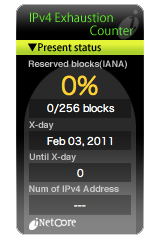
\includegraphics[height=6cm]{ipv4ec_iana_en.png}
\end{center}
\myurl{http://inetcore.com/project/ipv4ec/index_en.html}
\end{frame}

\begin{frame}
\frametitle{IPv6: Neuerungen}
\begin{itemize}
  \item \"Anderungen:
    \begin{itemize}
      \item Adressformat: $2^{128}=2^{32}\times 2^{32}\times 2^{32}\times 2^{32}$ seeeehr grosser Adressraum
      \item vereinfachte\footnote{in der Theorie\ldots viele Header sind ``optional'' und werden bei Bedarf eingef\"ugt (z.B. TCP-Header mit Portnummern, Sequenz, Flags)} Header/Metadaten
      \item keine Fragmentierung\footnote{ICMP6: ``packet too big''}
      \item Autokonfiguration durch ICMP6, ersetzt auch ARP
      \item ICMPv6 ``Autoconfiguration'' -- f\"ur Client-Hosts ohne DHCPv6\footnote{DHCP besteht weiterhin um z.B. in einem Firmennetz die Autokonfiguration zu unterdr\"ucken oder (Server-) Hosts mit einer fixen Adresse auszustatten}
      \item kein ARP -- wird durch ICMP6-Neighbor-Discovery\footnote{RFC-4861, mit L3-Multicast-Adressierung im Header!} abgel\"ost
    \end{itemize}
  \item bleibt gleich wie bei IPv4:
    \begin{itemize}
      \item Behandlung der ``upper layer'' Protokolle TCP/UDP, Portnummern bleiben gleich
    \end{itemize}
\end{itemize}
\end{frame}

\begin{frame}[fragile]
\frametitle{IPv6: Notation}
\begin{itemize}
  \item IPv6 wird in hexadezimaler Notation angegeben
  \item dabei werden jeweils 2 Bytes zusammengefasst und mit ``:'' getrennt $\rightarrow$ ergibt 8 Gruppen
  \item f\"uhrende Nullen in einer solchen Gruppe werden unterdr\"uckt
  \item die {\em l\"angste zusammenh\"angende} Sequenz von \texttt{:0:}-Gruppen kann mit ``::'' abgek\"urzt\footnote{das darf nur {\em einmal} pro IPv6-Adresse angewandt werden} werden
  \item Beispiel
    \begin{verbatim}
2001:41e0:ff00:01a3:0000:0000:0000:0002
2001:41e0:ff00:1a3:0:0:0:2
2001:41e0:ff00:1a3::2
    \end{verbatim}
\end{itemize}
\end{frame}

\begin{frame}[fragile]
\frametitle{IPv6: Adressraum}
IPv6 hat in Theorie $2^{128}$ Adressen, d.h. mehr als ausreichend in alle Ewigkeit -- \emph{aber} der Adressraum wird \"anlich wie bei IPv4 in Netz aufgeteilt
\begin{itemize}
   \item mit ganz ``kurzen'' Pr\"afixen wird eine Gruppierung nach ``link-local'', ``multicast'', ``global-unicast'', ``documentation-only''\footnote{\url{}http://www.iana.org/assignments/ipv6-address-space/ipv6-address-space.xml}} erreicht -- also eine Aufteilung nach technischem Verwendungszweck
   \item es werden ``regionale'' Pr\"afixe vergeben\footnote{Bestandteile der kurzen Pr\"afixe, eg. global-unicast}, zwischen /12 und /23 lang -- z.B. and ripe.net, arin.net, etc
	\item die Pr\"afixe der einzelnen Provider f\"ur Endkunden sind normalerweise zwischen /32 und /48 lang
	\item Endkunden bekommen im Normalfall ein /64 Netz, /48 ist aber auch kein Problem
\end{itemize}
...rechnen Sie mal die Anzahl Netzwerke/Hosts aus, die mit diesen Pr\"afixl\"angen m\"oglich sind!
\end{frame}



\begin{frame}
\frametitle{IPv6: Sicherheit}
\begin{itemize}
	\item IPv6 erm\"oglicht eine Verschl\"usselung auf L3-Ebene \"ahnlich wie IP-Sec bei v4 -- gut, aber aus Bequemlichkeit wird eher SSL (auf L4-7 Ebene) eingesetzt
	\item IPv6 ``global unicast'' sind auch durch einen Tunnel\footnote{d.h. egal von wo im Internet Sie sich verbinden} immer sichtbar -- \emph{kein} NAT-``Schutz'' mehr vorhanden\footnote{war eh nie als einziges Sicherheitselement gedacht}. Das wird viele Kunden und auch Hersteller von Endger\"aten zum Umdenken zwingen
	\item IPv6 Autokonfiguration kann nicht zwischen ``guten'' und ``b\"osen'' Routern unterscheiden
\end{itemize}
\end{frame}


\begin{frame}
\frametitle{IPv6: Autoconfiguration: Adressenformat EUI-64}
\begin{itemize}
  \item f\"ur Client-Hosts bietet sich die Link-Local Autoconfiguration an -- dabei wird an den vom Router gelieferten 64-Bit Pr\"afix eine ``erfundene'' 64-Bit Host-ID angeh\"angt\footnote{und nat\"urlich mit ICMP6-Neighbor-Solicitation gepr\"uft}
  \item Ohne ``privacy extensions'' wird der ``Host''-Teil der IPv6-Adresse normalerweise aus der MAC-Adresse gebildet
  \begin{center}
    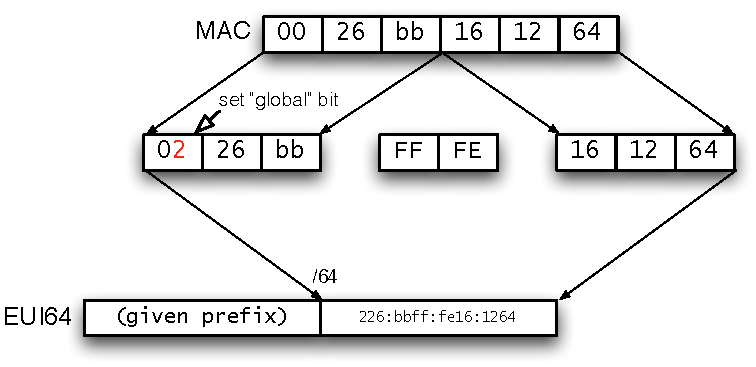
\includegraphics[height=4cm]{EUI64.pdf}
  \end{center}
  \item bei mobilen Clients werden diese 64 Bits immer gleich sein -- egal in welchem Netzwerk\footnote{IPv6 Hotspot, Provider, etc} $\rightarrow$ erm\"oglicht ein ``tracing'' eines Clients
\end{itemize}
\end{frame}

\begin{frame}
\frametitle{IPv6: Autoconfiguration: Privacy Extensions}
\begin{itemize}
  \item die ``privacy extensions''\footnote{RFC-4941} erzeugen f\"ur den 64-Bit-Host-Teil eine Zufallszahl\footnote{MD5 Hash}
  \item die so erzeugte Adresse wird nur einen bestimmten Zeitraum genutzt und dann durch eine neue ersetzt
  \item ``abgelaufene'' Adressen bleiben noch eine zeitlang aktiv, allerdings werden aktiv keine neuen Verbindungen mehr aufgebaut
\begin{block}{Privacy Extensions}
verhindert ``tracing''\footnote{die hintersten 48Bit w\"aren immer gleich der MAC des Ger\"ats} eines mobilen Clients durch diverse Netze
\end{block}
\end{itemize}
\end{frame}

\begin{frame}
\frametitle{IPv6: Autoconfiguration: IPv6-DHCP}
\begin{enumerate}
	\item Firmen m\"ochten nur bekannten Ger\"aten/Mitarbeitern einen Zugang zum Netz erm\"oglichen
	\item Benutzer m\"ochten verhindern, dass sie einem vorget\"auschten Router/b\"osen Hacker\footnote{die meisten sind lieb} auf den Leim gehen\footnote{der dann den ganzen Verkehr mith\"oren/\"andern k\"onnte}
\end{enumerate}
\begin{itemize}
  \item zentral gesteuerte/kontrollierte Vergabe\footnote{funktioniert genau gleich wie IPv4-DHCP} der IPv6-Adressen
  \item Client-Ger\"ate verbinden nicht mehr auf irgendwelche ``wilden'' Router\footnote{rouge access-points oder hier Router: wie im Internet-Cafe}
\end{itemize}
\end{frame}

\begin{frame}
\frametitle{IPv6: Anschlussm\"oglichkeiten}
\begin{itemize}
  \item ``native'' IPv6 -- wenn das lokale Netzwerk/Ihr Internet-Service-Provider bereits IPv6 unterst\"utzt und ins Internet routen kann
  \item ``tunnel'' IPv6: IPv6-Pakete werden irgendwie in IPv4-Pakete ``verpackt'' und so transportiert. Allen Modes gemeinsam: die MTU\footnote{Maximum-Transfer-Unit: Anzahl octets/bytes, die der L2 transportieren kann} wird um einen gewissen Betrag kleiner; braucht immer noch IPv4
     \begin{itemize}
        \item 6in4: ipv6-Paket wird als ganzes mit einem IPv4-Header\footnote{L3-protocol auf 41=ipv6 gesetzt. 6=TCP, 17=UDP. Probleme mit Firewalls/NAT} versehen, definiert in RFC4213\footnote{\url{http://tools.ietf.org/html/rfc4213}}
        \item Teredo: von Microsoft, benutzt IPv4-UDP\footnote{besser geeignet f\"ur NAT/Firewall}
        \item AYIYA: ``anything in anything': ``eingepacktes'' und ``transport''-Protokoll frei w\"ahlbar. Meistens in Verbindung mit ``automatischer'' Konfiguration. {\tiny Versuchen Sie es selbst: \url{https://www.sixxs.net/}}
	\item ``mobile-IPv6'': kann theoretisch ohne Tunnel effizient mobile/\"andernde IPv6-Adressen einer festen/globalen Adresse zuweisen\footnote{weniger im Gebraucht, braucht totale Durchdringung mit IPv6 in der Infrastruktur}
     \end{itemize}
\end{itemize}
\end{frame}

\begin{frame}
\frametitle{IPv6: DNS}
wird einerseits \"uber IPv6 angeboten und andernseits wurde ein neuer Resource-Record-Typ eingef\"uhrt:
\begin{itemize}
	\item Hostname$\rightarrow$IPv6: \texttt{zaphod		IN AAAA		2a01:4f8:100:41e6::2}
	\item IPv6$\rightarrow$Hostname: Ok, das ist h\"asslich:\\ {\tiny \texttt{2.0.0.0.0.0.0.0.0.0.0.0.0.0.0.0.6.e.1.4.0.0.1.0.8.f.4.0.1.0.a.2.ip6.arpa. IN PTR zaphod.netlabs.ch.}}
\end{itemize}
\end{frame}


\begin{frame}
\frametitle{IPv6: weshalb gibt's seit 10 Jahren\footnote{+/-} einen ``Launch Day''?}
\begin{itemize}
	\item Internet-Service-Provider sind eigentlich alle bereit (besonders die ``h\"oher'' in der ``Hierarchie'')
	\item Endkunden-Service-Provider (swisscom, sunrise, green, etc) z\"ogern noch -- die Anbindung ans Internet ist kein Problem aber die Verwaltung der Endkundenger\"ate bedeutet einige Umstellung
	\item wenig bis gar kein Druck seitens der Endkunden/Benutzer und der Content-Provider (Firmen, etc)
\end{itemize}
\end{frame}





\begin{frame}
\frametitle{IPv6: Einrichten IPv6 Tunnel}
\begin{itemize}
  \item Tunnel-Broker\footnote{reserviert ein pers\"onliches IPv6 subnet f\"ur Sie und verwaltet das Routing auf einen POP/Tunnel-Provider} ausw\"ahlen (f\"ur 6in4
  \item auf dem Endsystem {\texttt aiccu}\footnote{ein \em{AIYIA} Anything-In-Anything Protokoll} installieren
\end{itemize}
\end{frame}


\end{document}
